Most of the processes the robot is doing need either to get some information from external sensors or to send data to the actuators or displays. This is useful in the two ways of the communication. Sensors will give information to the robot so it can sense better the environment and act in consequence of what is happening in the \textit{exterior} world. Actuators, or output peripherals, give feedback to the persons interacting with the robot. Imagine for example explaining some instructions in an LCD screen or playing some sounds in certain actions of the robot. This will make the interaction easier and a more reach experience. Whenever it is needed to communicate with external devices, the robot needs to use drivers.

During this part the sound and LCD modules will be explained as output devices and ultrasonic sensor as input device. It is important to remark that, although the motion module is run using drivers, it will not be explained in this section since a special section is dedicated to it due its importance.

A driver is non other than a small program that allows a computer (in the current case a Raspberry Pi) to communicate with some external devices. It gives basic instructions and functions to make an easy interaction between the both parts.

In this point it is important to remark two different groups of devices. The first one includes the sound module, which is already built in the Raspberry Pi. This makes it easy to simply just plug a speaker using a 3.5mm jack. The second group, formed by the ultrasonic sensor and the LCD screen need an $I^{2}C$ protocol in order to communicate with the RPi.

For the first module it is only needed an external speaker that can be easily plugged with a standard jack. In this case the Raspberry Pi already provides support for launching different sounds so it is straight forward to make it work. For example whenever the button of the robot is pressed a sound is played in order to give feedback to the children about the starting or shutting down of the program. The program that controls the button is written in \textit{Python} and an instruction like \lstinline{os.system('omxplayer song.mp3')} reproduces a sound.

In the second group a new protocol is introduced: $I^{2}C$, that refers to \textit{Inter Integrated Circuit}, a multi-master and multi-slave serial bus. It is a protocol used for attaching low-speed peripherals to embedded systems, small computers or microchips. The power of $I^{2}C$ is that allows to connect several devices in the same line of cables. By identifying each one of this devices by a unique address it is possible to control all of them. In figure \ref{fig:i2c} it is possible to observe the connection of the two devices that make use of $I^{2}C$. As can be seen only four cables are needed for sending and receiving data. Red and black are used as power source, typically +5V or +3.3V. Green and blue cables are Serial Data Line (SDA) and Serial Clock Line (SCL). The working principle of $I^{2}C$ is very easy. Each one of the devices has a specific address which is known a priori (certain addresses are available to chose for each device). When it is needed to communicate with one of them a buffer is sent to the correspondent address and the device acts in consequence. Later it is explained each one how it works.

\begin{figure}[h]
\centering
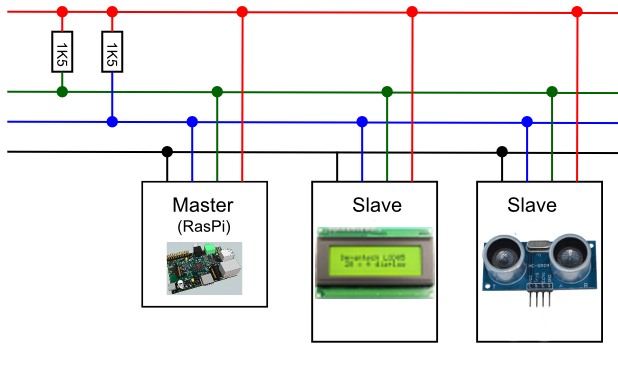
\includegraphics[width = 0.6\textwidth]{i2c}
\caption{Connection of multiple devices to a $I^{2}C$ port. Raspberry Pi is working as master while the other two peripherals are working as slave.}
\label{fig:i2c}
\end{figure}


LCD display is used in order to show information about the current state of the robot. Is a very powerful way to know what the robot is thinking or doing without the need of connecting a screen to the Raspberry Pi. This is very important since the less computational power expended on the RPi the better. Avoiding the initialization of a graphical user interface will result in a slightly more fast execution of the program, which is desired. It is also a very nice way to communicate with children and explain maybe some instructions or the current state of the robot so they know what the robot is doing. The flow of the information in the $I^{2}C$ bus is only in one way, from the RPi to the LCD. Whenever it is needed to write something in the screen a command is sent via the bus and the device executes it. The two most common functions used are the ones to write and clean the screen.

Proximity sensor will give information to the robot about its surroundings. The working principle is based on ultrasonic sounds that rebound on objects. By calculating the amount of time for a sound wave to get back to the sensor it is possible to estimate the distance. In this case the $I^{2}C$ bus is working in two directions. In order to get data from the sensor first it is need to send some information to it. It is like a conversation where the RPi asks for information and the ultrasonic sensor responds with this data.In this way it is avoided to continuously receive unnecessary data. Grabbing distance two or three times per second is enough in the current case since the robot is not moving fast.
